\documentclass[tikz]{standalone}

\usepackage{pgfplots}
\pgfplotsset{compat = newest}
\usepgfplotslibrary{statistics}

\begin{document}
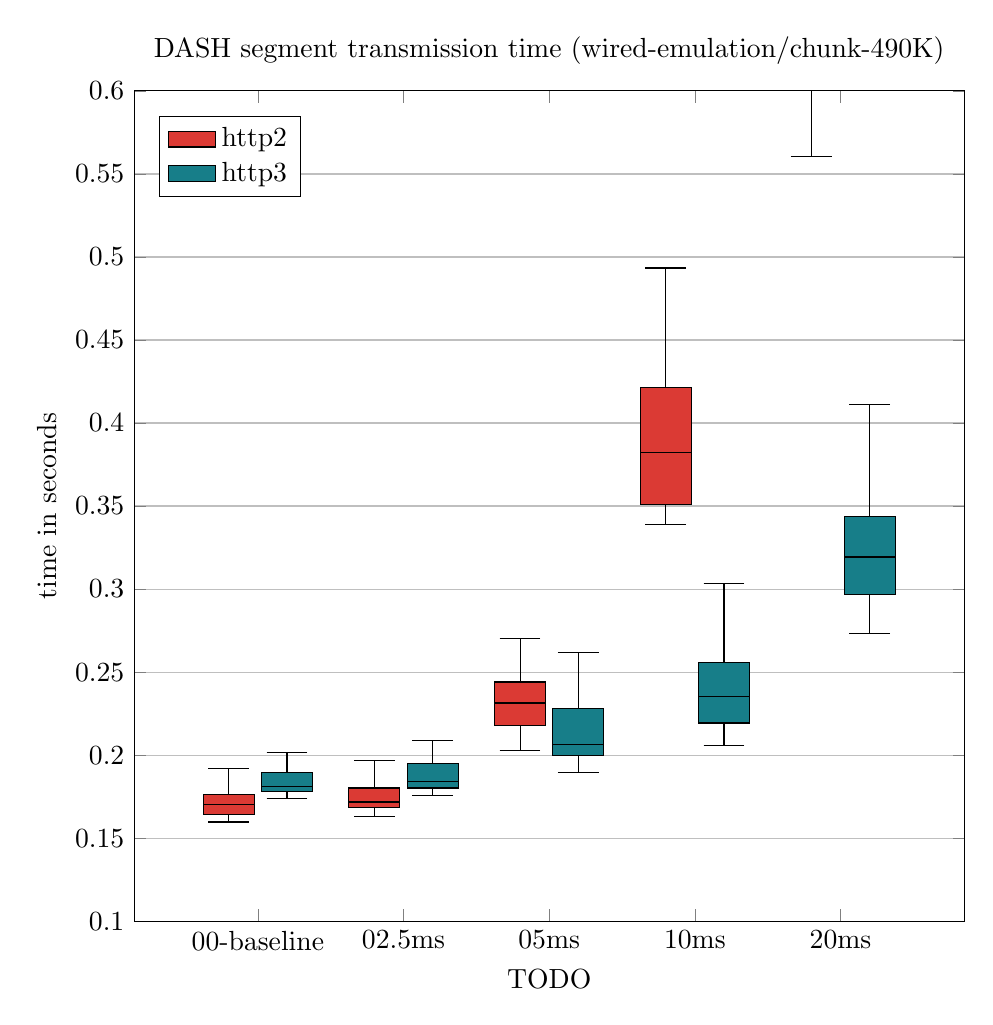
\begin{tikzpicture}

\definecolor{red}{RGB}{219,58,52}
\definecolor{blue}{RGB}{23,126,137}

\begin{axis}
[
    title={DASH segment transmission time (wired-emulation/chunk-490K)},
    xlabel={TODO},
    ylabel={time in seconds},
    xtick={1,2,3,4,5},
    xticklabels={00-baseline,02.5ms,05ms,10ms,20ms},
    ymin=0.1,
    ytick distance=0.05,
    ymax=0.6,
    boxplot/box extend=0.35,
    boxplot/draw direction=y,
    area legend,
    legend entries={http2, http3},
    legend pos=north west,
    ymajorgrids = true,
    yminorgrids = true,
    major grid style = {lightgray},
    minor grid style = {lightgray!25},
    width = \textwidth,
    height = \textwidth,
]

% START PLOTS

\addplot+[
fill=red,
draw=black,
solid,
boxplot prepared={
    draw position=0.8,
    lower whisker=0.15969561000019894,
    lower quartile=0.16404166249958507,
    median=0.17017334299998765,
    upper quartile=0.17634600249948562,
    upper whisker=0.19208022499879007
},
] coordinates {};
% ] coordinates {(0,0.3051776879983663) (0,0.2917083669999556) (0,0.288851152999996) (0,0.20956114100044942) (0,0.2843116430012742)};
\addplot+[
fill=blue,
draw=black,
solid,
boxplot prepared={
    draw position=1.2,
    lower whisker=0.1739389829999709,
    lower quartile=0.1779343255002459,
    median=0.18102312399969378,
    upper quartile=0.189650747000087,
    upper whisker=0.20154879499932576
},
] coordinates {};
% ] coordinates {(0,0.2116752340007224) (0,0.2202450040003896) (0,0.21183131799989496) (0,0.33470439200027613) (0,0.20820489300058398) (0,0.22703768700012006) (0,0.32479370399960317) (0,0.3203285279996635)};
\addplot+[
fill=red,
draw=black,
solid,
boxplot prepared={
    draw position=1.8,
    lower whisker=0.16303114000038477,
    lower quartile=0.16832654750123766,
    median=0.17173890999947616,
    upper quartile=0.18022653400021227,
    upper whisker=0.19699092699920584
},
] coordinates {};
% ] coordinates {(0,0.29119598499892163) (0,0.2805090010006097) (0,0.20021539400113397) (0,0.30400489100065897) (0,0.3065033980001317) (0,0.3492119170005026) (0,0.22122611199847597) (0,0.22579149800003506) (0,0.2426118300008966) (0,0.20811137199962104) (0,0.3011856789999001)};
\addplot+[
fill=blue,
draw=black,
solid,
boxplot prepared={
    draw position=2.2,
    lower whisker=0.17560691400103678,
    lower quartile=0.18020421549954335,
    median=0.18408205800005817,
    upper quartile=0.19476472950009338,
    upper whisker=0.2085628650002036
},
] coordinates {};
% ] coordinates {(0,0.225894822000555) (0,0.31938245999845094) (0,0.3171744969986321) (0,0.29952866500025266) (0,0.24110111099980713) (0,0.23550447300112864) (0,0.2586941939989629) (0,0.22408777899909182)};
\addplot+[
fill=red,
draw=black,
solid,
boxplot prepared={
    draw position=2.8,
    lower whisker=0.20261520700114488,
    lower quartile=0.21808928599966748,
    median=0.2313774439990084,
    upper quartile=0.24403805899964937,
    upper whisker=0.27015899700018053
},
] coordinates {};
% ] coordinates {(0,0.3518833639991499) (0,0.3868573669988109) (0,0.3320103999994899) (0,0.3682998240001325)};
\addplot+[
fill=blue,
draw=black,
solid,
boxplot prepared={
    draw position=3.2,
    lower whisker=0.18930091899892432,
    lower quartile=0.2000227155003813,
    median=0.2061784590005118,
    upper quartile=0.22813209749983798,
    upper whisker=0.26182855300066876
},
] coordinates {};
% ] coordinates {(0,0.3527831480005261) (0,0.2713931589987624) (0,0.28251568599989696) (0,0.313206552000338) (0,0.3436451270008547) (0,0.34281166899927484)};
\addplot+[
fill=red,
draw=black,
solid,
boxplot prepared={
    draw position=3.8,
    lower whisker=0.3388278000002174,
    lower quartile=0.3509587489998012,
    median=0.38228420300038124,
    upper quartile=0.42158121799911896,
    upper whisker=0.4933498110003711
},
] coordinates {};
% ] coordinates {(0,0.5390700520001701)};
\addplot+[
fill=blue,
draw=black,
solid,
boxplot prepared={
    draw position=4.2,
    lower whisker=0.20591256099942257,
    lower quartile=0.21933332299977337,
    median=0.23511317399970721,
    upper quartile=0.2558023725005114,
    upper whisker=0.303121638000448
},
] coordinates {};
% ] coordinates {(0,0.42226239400042687) (0,0.4208558480004285) (0,0.3818508770000335) (0,0.4096933649998391) (0,0.3817935030001536)};
\addplot+[
fill=red,
draw=black,
solid,
boxplot prepared={
    draw position=4.8,
    lower whisker=0.5603062249992945,
    lower quartile=0.6405631499992523,
    median=0.7144828559994494,
    upper quartile=0.7265386200006105,
    upper whisker=0.8198880750005628
},
] coordinates {};
% ] coordinates {(0,0.4861180779989809) (0,0.9122208610006055) (0,0.9035316329991474)};
\addplot+[
fill=blue,
draw=black,
solid,
boxplot prepared={
    draw position=5.2,
    lower whisker=0.2731243060006818,
    lower quartile=0.29684907750015554,
    median=0.3193276780002634,
    upper quartile=0.34380332349974196,
    upper whisker=0.41132956799992826
},
] coordinates {};
% ] coordinates {(0,0.581385280998802) (0,0.49803008699927886) (0,0.45658193300005223) (0,0.4441399150000507) (0,0.41465498999968986) (0,0.4411014569996041)};
% END PLOTS

\end{axis}
\end{tikzpicture}
\end{document}